% ResearchPhO question paper template: strict IPhO/APhO theory format (compile twice with pdflatex).
% The question paper contains ONLY: general instructions, problems (introduction, figures, given data,
% useful information, parts, boxed subquestions with points). No status frames, sources boxes, research notes.
\documentclass[11pt,a4paper]{article}
\usepackage[T1]{fontenc}
\usepackage[utf8]{inputenc}
\usepackage{fix-cm}
\usepackage[scaled=0.96]{helvet}
\renewcommand{\familydefault}{\sfdefault}
\usepackage{amsmath,amssymb,mathtools}
\usepackage{newtxmath}
\usepackage{bm,dsfont}
\usepackage[margin=20mm,top=35mm,bottom=20mm,headheight=57pt,headsep=10mm]{geometry}
\usepackage{microtype,booktabs,array,tabularx,enumitem,needspace}
\usepackage[most]{tcolorbox}
\usepackage{fancyhdr,xcolor}
\usepackage{tikz}
\usetikzlibrary{arrows.meta,calc,positioning}
\usepackage{pgfplots}
\pgfplotsset{compat=1.18}
\usepackage[hidelinks,pdfencoding=auto,psdextra]{hyperref}
\definecolor{ink}{HTML}{172A3A}
\definecolor{rulegray}{HTML}{5E6670}
\definecolor{colA}{HTML}{D9822B}
\definecolor{colB}{HTML}{3C78B4}
\setlength{\parindent}{0pt}
\setlength{\parskip}{5.4pt}
\setlength{\emergencystretch}{2em}
\raggedbottom
% ---------------- page codes: G-n on the cover, T<problem>-n inside problem <problem> ----------------
\newcounter{problemno}
\newcounter{figc}
\renewcommand{\thefigc}{\arabic{problemno}.\arabic{figc}}
\newcommand{\pagecode}{G}
\renewcommand{\thepage}{\pagecode-\arabic{page}}
\pagestyle{fancy}
\fancyhf{}
\fancyhead[L]{\begin{minipage}[b]{0.73\textwidth}\textbf{\large Theory}\\[-1pt]{\small ResearchPhO \enspace|\enspace Questions}\\[-1pt]{\footnotesize English}\end{minipage}}
\fancyhead[R]{\fontsize{29}{31}\selectfont\bfseries \thepage}
\renewcommand{\headrulewidth}{0.9pt}
\fancyfoot[L]{\footnotesize ResearchPhO --- a research-based exam in IPhO/APhO format; not an official olympiad paper}
% ---------------- notation ----------------
\newcommand{\ket}[1]{\lvert #1\rangle}
\newcommand{\bra}[1]{\langle #1\rvert}
\newcommand{\Tr}{\operatorname{Tr}}
\newcommand{\dd}{\mathrm d}
\newcommand{\norm}[1]{\left\lVert #1\right\rVert}
\newcommand{\id}{\mathds 1}
% ---------------- structure ----------------
% \problem{number}{title}{points}: new page, page code T<number>, figure numbers <number>.k
\newcommand{\problem}[3]{\clearpage\setcounter{problemno}{#1}\renewcommand{\pagecode}{T#1}\setcounter{page}{1}\setcounter{figc}{0}{\LARGE\bfseries\color{ink}Problem #1: #2}\hfill{\large\bfseries(#3 points)}\par\medskip}
\newcommand{\parttitle}[3]{\par\Needspace{8\baselineskip}\vspace{6pt}{\large\bfseries\color{ink}Part #1. #2\hfill\normalsize(#3 points)}\par\vspace{2pt}}
\newcommand{\smallheading}[1]{\par\Needspace{6\baselineskip}\medskip\textbf{#1}\par}
% \question{label}{points}{text}: boxed subquestion; use \textbf{(a)}, \textbf{(b)} for sub-parts
\newcommand{\question}[3]{\begin{tcolorbox}[enhanced,colback=white,colframe=rulegray,boxrule=0.5pt,arc=0pt,left=7pt,right=7pt,top=7pt,bottom=7pt,before skip=9pt,after skip=9pt]\begin{tabularx}{\linewidth}{@{}>{\bfseries}p{10mm}X>{\raggedleft\arraybackslash}p{13mm}@{}}#1&#3&\textbf{#2 pt}\end{tabularx}\end{tcolorbox}}
\newcommand{\hint}[1]{\par{\small\textbf{Hint.} #1}\par}
% plain numbered figure: \begin{figpanel}{short title} tikz \figtext{description} \end{figpanel}
\newenvironment{figpanel}[1]{\refstepcounter{figc}\gdef\figtitle{#1}\par\medskip\noindent\begin{minipage}{\linewidth}\centering}{\end{minipage}\par\medskip}
\newcommand{\figtext}[1]{\par\smallskip{\raggedright\small\textbf{Figure \thefigc.} \figtitle. #1\par}}
\newcolumntype{Y}{>{\raggedright\arraybackslash}X}
\tikzset{>={Stealth[length=2.2mm]}}
\pgfplotsset{mbaxis/.style={width=7.6cm,height=5.4cm,tick label style={font=\scriptsize},label style={font=\small},axis line style={rulegray},tick style={rulegray}}}
% ==== BEGIN GENERATED FIGURE DATA (your script) ====
\newcommand{\FigDataExample}{\addplot[colB,thick] coordinates {(0,0) (0.5,0.4) (1,0.6) (1.5,0.7) (2,1.0)};}
% ==== END GENERATED FIGURE DATA ====
\begin{document}

{\LARGE\bfseries\color{ink}TITLE OF THE EXAM}\par
{\large ResearchPhO --- Theoretical examination \hfill \textbf{30 points}}

\smallheading{General instructions}
\begin{enumerate}[leftmargin=7mm,itemsep=3pt]
\item The theoretical examination lasts 5 hours. It has three problems; each problem is worth 10 points.
\item You may use a non-programmable scientific calculator. No other aids are allowed.
\item Write each final answer in the box with the same label on the Answer Sheet of that problem. Use blank writing sheets for derivations you want graded.
\item Write on the front side of the sheets only. Use equations, numbers, symbols and diagrams rather than words.
\item The problems are independent and can be solved in any order.
\end{enumerate}

\smallheading{Problems}
{\small\begin{tabularx}{\textwidth}{@{}p{18mm}Y r@{}}\toprule
Problem&Title&Points\\\midrule
1&FIRST PROBLEM&10.0\\
2&SECOND PROBLEM&10.0\\
3&THIRD PROBLEM&10.0\\\midrule
&&\textbf{30.0}\\\bottomrule
\end{tabularx}}

\problem{1}{FIRST PROBLEM}{10.0}
Introduction in plain words: the system, the phenomenon, why it matters. Explain every concept that is not in the
IPhO syllabus in terms of syllabus physics. State the model and all conventions here.

\begin{figpanel}{The system}
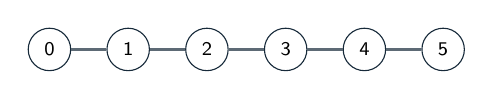
\begin{tikzpicture}[x=10mm,y=10mm]
\foreach \x in {0,...,5}{\node[circle,draw=ink,minimum size=5mm,font=\scriptsize] (n\x) at (\x,0) {\x};}
\foreach \x [evaluate=\x as \y using int(\x+1)] in {0,...,4}{\draw[ink!70,line width=1pt] (n\x)--(n\y);}
\end{tikzpicture}
\figtext{A plain description of what is drawn; no answers.}
\end{figpanel}

\smallheading{Useful information}
\begin{itemize}[leftmargin=6mm,itemsep=2pt]
\item Only the facts this problem needs, each in one line.
\end{itemize}

\parttitle{A}{FIRST PART}{4.0}
Context and given data for Part A.
\question{A.1}{1.5}{Find \dots. Explain \dots.}
\question{A.2}{2.5}{\textbf{(a)} Derive \dots.\par \textbf{(b)} Show \dots.}
\hint{Name the tool, not the step.}

\parttitle{B}{SECOND PART}{6.0}
\begin{figpanel}{A computed picture}
\begin{tikzpicture}
\begin{axis}[mbaxis,xlabel={$t/T$},ylabel={quantity}]
\FigDataExample
\end{axis}
\end{tikzpicture}
\figtext{Computed from the model; state its scope.}
\end{figpanel}
\question{B.1}{6.0}{Evaluate \dots.}

\problem{2}{SECOND PROBLEM}{10.0}
Each problem starts with its own introduction and can be solved without the others.
\parttitle{A}{FIRST PART}{10.0}
\question{A.1}{10.0}{\dots}

\problem{3}{THIRD PROBLEM}{10.0}
\parttitle{A}{FIRST PART}{10.0}
\question{A.1}{10.0}{\dots}

\vfill
\begin{center}\textbf{End of the theoretical examination}\end{center}
\end{document}
